We will find the current response of a single Dirac cone, with a temperature gradient $\nabla_y T$ and a magnetic field $B_z$.
The current response of interest in the given geometry is thus in the $x$-direction,
\begin{equation}\label{eq:3}
  J^x = \chi ^{xy} \frac{- \nabla _yT}{T},
\end{equation}
with $\chi^{xy}$  being the response\footnote{The sign in Eq. (\ref{eq:3}) depends on the choice of the response function being the response of the gravitational potential or the temperature gradient. Thus, the sign may differ in the literature.}.
This geometry is shown in Figure \ref{fig:setup}.
\begin{figure}[ht]
  \centering
  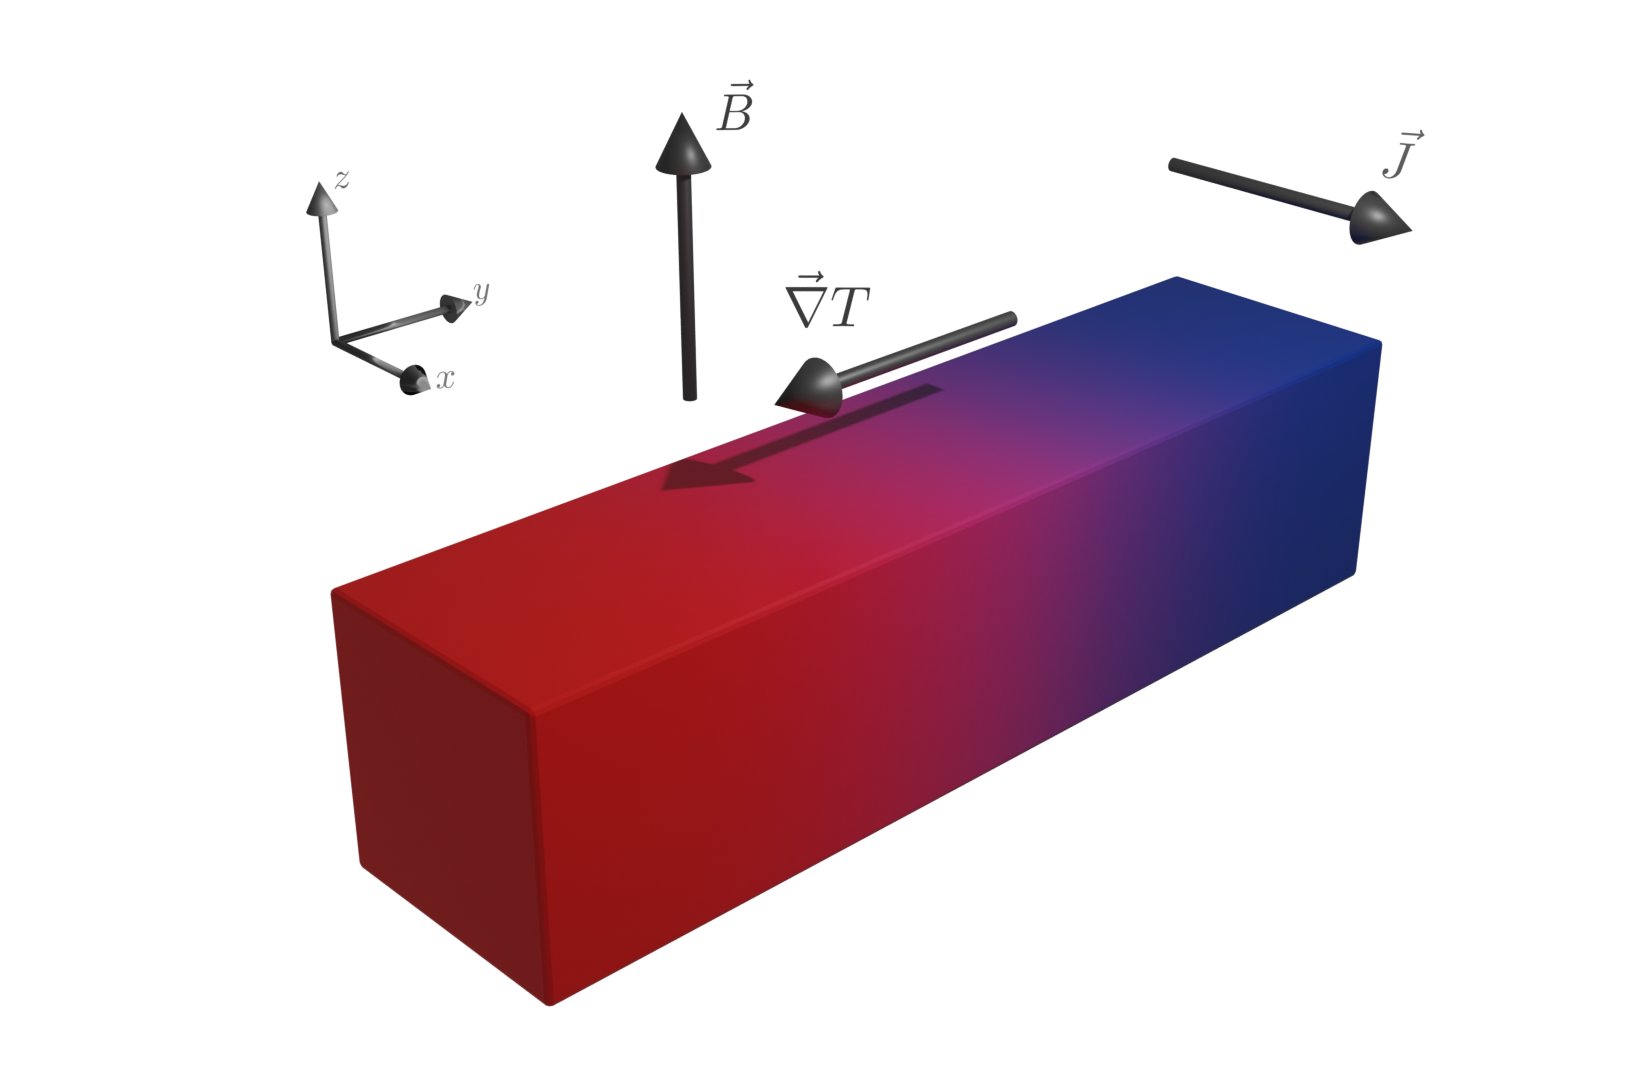
\includegraphics[width=0.7\textwidth]{figures/setup.png}
  \caption{Sketch of the geometry used in the derivation. Note that we consider only bulk response, and the finite sample is only for illustration purposes. \label{fig:setup}}
\end{figure}
In the derivation of~\citeauthor{chernodubGenerationNernstCurrent2018}~\cite{chernodubGenerationNernstCurrent2018} the response
\begin{equation}
  \chi ^{xy} = \frac{e^2 v_F B}{18 \pi ^2 \hbar }
\end{equation}
was found, while the derivation of~\citeauthor{arjonaFingerprintsConformalAnomaly2019}~\cite{arjonaFingerprintsConformalAnomaly2019} found
\footnote{The paper is somewhat unclear on what is their final result, as there is some possible confusion related to the number of Landau levels included and whether one is including both or only one Dirac cone.
The above result is what is meant, to the best of our understanding.}
\begin{equation}
  \chi ^{xy} = \frac{e^2 v_F B}{4 \pi ^2 \hbar }.
\end{equation}

Recall the linear response from the Kubo formalism in Eq. (\ref{eq:current-luttinger-gravity-final}), found through Luttinger's approach.
\begin{equation}
  \label{eq:4}
  \braket{J^i}(t, \vec{r}) =
  \int\limits_{-\infty }^{\infty } \mathrm{d}t' \mathrm{d}\vec{r}'
  \int\limits_{-\infty }^{t'} \mathrm{d}t''
  \left\{
    \frac{-i v_F}{\hbar } \Theta (t-t')
    \Braket{
      [J^i(t, \vec{r}), T^{0j} (t'', \vec{r}')]
    }
  \right\}
  \partial _j' \psi (t', \vec{r}').
\end{equation}
Fourier transforming now to the frequency and momentum domain, will be beneficial in our calculations.
As before, the non-perturbed system will be taken to be time and position invariant, such that the correlator in Eq. (\ref{eq:4}) can be taken to depend only on the differences $t-t''$ and $\vec{r} - \vec{r}' $.
Starting with Fourier transforming the position part, notice that the structure of Eq. (\ref{eq:4}) is
\[
  \braket{J^i}(\vec{r}) = \int \mathrm{d} \vec{r}' \chi (\vec{r} - \vec{r}') \partial _j' \psi  (\vec{r}'),
\]
where the temporal parts were dropped for clarity.
This is a convolution, and the Fourier transform is thus simply given by the product of the two factors~\cite{rottmannMatematiskFormelsamling1995}.
\begin{equation}
  \braket{J^i}(\vec{q}) =
  \chi (\vec{q}) (iq_j) \psi (\vec{q}),
\end{equation}
where it was also used that the Fourier transform of a derivative gives the component of the variable.
Showing explicitly how to find the form of the response $\chi $ in momentum space is often overlooked in much literature, and as it does involve some finesse, we want to show it here.
This trick is courtesy of~\citeauthor{changLectureNotesManybody2018}~\cite{changLectureNotesManybody2018}.
By definition, the Fourier transform of the response is, where the variable of integration has been chosen to be $\vec{r}-\vec{r}'$ for later convenience,
\begin{align}
  \chi (\vec{q}) &= \int \mathrm{d}(\vec{r} - \vec{r}') e^{-i\vec{q}(\vec{r}-\vec{r}')} \chi (\vec{r} - \vec{r}')\\
                 &= \int \mathrm{d}(\vec{r} - \vec{r}') e^{-i\vec{q}(\vec{r}-\vec{r}')} C \Braket{
                   \left[
J^i (\vec{r}), T^{0j}(\vec{r}')
                   \right]},\\
\end{align}
where $C$ denotes $t$-dependent prefactors and integrals over time are omitted, again for clarity of notation.
Note that
\begin{equation}
  \int \mathrm{d}(\vec{r} - \vec{r}') = \frac{1}{\mathcal{V}} \int \mathrm{d}\vec{r} \mathrm{d} \vec{r}',
\end{equation}
where $\mathcal{V}$ is the volume of the system.
Thus,
\begin{equation}
  \begin{split}
    \chi (\vec{q}) &= \frac{1}{\mathcal{V}} \int \mathrm{d}\vec{r} \mathrm{d}\vec{r}'
    e^{-i\vec{q}(\vec{r}-\vec{r}')}
    C \Braket{\left[
        J^i(\vec{r}), T^{0j}(\vec{r}')
      \right]}\\
    &= \frac{C}{\mathcal{V}} \Braket{\left[ J^i(\vec{q}), T^{0j}(-\vec{q}) \right]}.
  \end{split}
\end{equation}

Considering now the temporal part, the procedure is simpler.
The linear response still has the form of a convolution, as the response function is only dependent on the difference $t-t'$ by
\begin{equation}
  \chi (t-t') = \int\limits_{-\infty }^0 \mathrm{d} t'' \Theta (t - t')
  \Braket{\left[ J(t-t'), T(t'') \right]},
\end{equation}
where $t''$ was shifted by $t' $, and then the translational invariance of the correlator was used.
In frequency space
\begin{align}
  \chi (\omega ) &= \int \mathrm{d} t e^{i \omega  t} \chi (t)\\
                 &= \int \mathrm{d} t e^{i \omega  t} \int\limits_{-\infty  }^0 \mathrm{d} t''
                   \Theta (t) \Braket{\left[ J(t), T(t'') \right]}.
\end{align}
In frequency and momentum space the response function is thus
\begin{equation}\label{eq:5}
  \chi ^{ij} (w, \vec{q}) =
  \frac{-iv_F}{\mathcal{V} \hbar } 
  \int \mathrm{d}t e^{i\omega t}
  \int\limits_{-\infty }^{0} \mathrm{d}t'
  \Theta (t)
  \Braket{\left[
      J^i(t, \vec{q}), T^{0j}(t', -\vec{q})
    \right]}.
\end{equation}

\section{Eigenvalue problem of the Landau levels of a Weyl Hamiltonian}
To evaluate the correlator of the response function, the matrix elements of the current and stress-energy tensor must be found.
In order to do this, we find eigenstates in the Landau basis of the system.
The Weyl Hamiltonian
\begin{equation}
  \label{eq:weyl-hamil}
  H_s = s v_F \sigma^i \left( p_i + e A_i \right),
\end{equation}
with $s$ being the chirality, $p_i$ the momentum operator, and $e = |e|$ the coupling constant to the electromagnetic field $\vec{A}$.
Choose coordinates such that $\vec{B} = B_z \hat{\vec{z}}$, which in the Landau gauge gives $\vec{A} = -B_{z}y \: \hat{\vec{x}}$.
As the Hamiltonian is invariant in $x$ and $z$, take the plane wave ansatz $\phi(\vec{r}) = e^{ik_x x + i k_z z} \phi (y)$.
It then follows
\begin{equation}
  H_s \phi(\vec{r}) = E \phi(\vec{r}) \implies \tilde{H}_s \phi(y)  = E \phi(y),
\end{equation}
where $\tilde{H}$ is the result of replacing $p_z \to \hbar k_z, p_x\to \hbar  k_x$ in $H_s$, as the plane wave part of $\phi $ have these eigenvalues.
Absorb the chirality $s$ as a sign in the velocity $v_F$, for more concise notation. 
Thus, writing everything explicitly, the spectrum is given by
\begin{equation}
  \label{eq:6}
  -\hbar  v_F
  \begin{pmatrix}
    - k_z & \partial _y + e y B_{z} / \hbar  - k_x\\
    -\partial _y + e y B_{z} / \hbar -k_x & k_z
  \end{pmatrix}
  \phi(y)  = E\phi(y).
\end{equation}
We will now find the spectrum $E$ of the Hamiltonian.

Inspired by the derivation for the spectrum of the 2D Dirac Hamiltonian in~\cite{wehlingDiracMaterials2014}, we introduce the length scale $l_B = \sqrt{\hbar / eB}$, and the dimensionless quantity $\chi = y /l_{B} - k_x l_{B}$.
In dimensionless quantities Eq. (\ref{eq:6}) becomes
\begin{equation}
  -\frac{{\hbar v_F}}{l_{B}}
  \begin{pmatrix}
    -k_z l_B & \partial _{\chi } + \chi \\
    -\partial _{\chi } + \chi & k_z l_B
  \end{pmatrix}
  \phi(y)  =  E \phi(y).
\end{equation}
Let the operators \(a = \left( \chi + \partial _{\chi } \right) / \sqrt{2},\; a^{\dagger} = \left( \chi - \partial _{\chi } \right) /\sqrt{2}\).
One may easily verify the commutation relation $[a, a^{\dagger}] = 1$;
they are ladder operators of the harmonic oscillators, whose eigenstates are $\ket{n}$, and where $a\ket{n} = \sqrt{n}\ket{n-1}, a^{\dagger} \ket{n} = \sqrt{n+1} \ket{n+1}$.
In terms of these operators, the system is
\begin{equation}
  -\frac{\sqrt{2} \hbar v_F}{l_B}
  \begin{pmatrix}
    -\frac{k_zl_B}{\sqrt{2}} & a\\
    a^{\dagger} & \frac{k_zl_B}{\sqrt{2}}
  \end{pmatrix}
  \ket{\phi } = E \ket{\phi }.
\end{equation}
Take the ansatz
\begin{equation}
  \ket{\phi } =
  \begin{pmatrix}
    \beta \ket{n-1}\\
    \alpha  \ket{n}
  \end{pmatrix},
\end{equation}
which is the most general form of $\ket{\phi }$ with any hope of being an eigenstate.
This leads to
\begin{equation}
  -\frac{\sqrt{2} \hbar v_F}{l_B}
  \begin{pmatrix}
    \left( -\gamma \beta + \alpha \sqrt{n} \right) \ket{n-1}\\
    \left( \beta \sqrt{n} + \gamma \alpha \right) \ket{n}
  \end{pmatrix}
  = E \ket{\phi },
\end{equation}
with $\gamma  = k_zl_B / \sqrt{2}$.
For $n > 0$ this leads to the equation for $\phi $ to be an energy eigenfunction
\begin{equation}
  -\gamma + \frac{\alpha}{\beta } \sqrt{n} = \frac{\beta }{\alpha } \sqrt{n} + \gamma.
\end{equation}
Solving for $\alpha /\beta $ this gives
\begin{equation}
  \frac{\alpha}{\beta } = \frac{\gamma}{\sqrt{n}} \pm \sqrt{1 + \frac{\gamma^2}{n}},
\end{equation}
and thus
\begin{equation}
  E = \pm v_F \sqrt{
    \frac{2n \hbar ^2}{l_B^2} + k_z^2\hbar ^2
  }
  = \pm s v_F \sqrt{
    2n e B \hbar + k_z^2\hbar ^2
  },
\end{equation}
where we reintroduced the explicit $s$.
For $n = 0$ the annihilation operator $a$ destroys the vacuum state $\ket{0}$, and the energy is instead $E_0 = -\hbar s k_z v_F$.
The excited energy states are doubly degenerate;
we choose to denote the energy levels by $m \in \mathbb{Z}$, where the sign from $\pm s$ is taken care of by the sign of this quantum number, and the harmonic oscillator levels $n$ are given by its absolute value $|m|$.
The energy levels are
\begin{align}
  E_{k_z m s} &= \operatorname{sign}(m) v_F \sqrt{2 |m| e B \hbar  + k_z^2 \hbar ^2} & \text{ for } m \neq 0,\\
E_{k_z 0 s} &= -s \hbar k_z v_F & \text{ for } m = 0.
\end{align}

We now find the corresponding eigenvectors of the system.
The solution to the one dimensional harmonic oscillator in position space is, in dimensionless coordinates $\xi$,~\cite[Eq.~18.39.5]{NIST:DLMF}
\begin{equation}
  \braket{\xi | n} = \phi _n (\xi)
  = \frac{1}{\sqrt{2^nn!}} \pi^{-\frac{1}{4}}
  e^{- \frac{\xi^2}{2}} H_n \left( \xi \right),
  % = \frac{1}{\sqrt{2^nn!}} \left( m\frac{\omega}{\pi \hbar } \right)^{\frac{1}{4}}
  % e^{- \frac{{m\omega x^2}}{2\hbar }} H_n \left( \sqrt{\frac{m\omega }{\hbar } x} \right),
\end{equation}
where $H_n$ are the Hermite polynomials.
Thus,
\begin{equation}
  \braket{\chi | \phi } =
  \begin{pmatrix}
    \beta \braket{\chi | n-1}\\
    \alpha \braket{\chi | n}
  \end{pmatrix}
  =
  e^{- \frac{\chi^2}{2}}
  \begin{pmatrix}
    \frac{\beta }{\sqrt{2^{n-1}(n-1)!\sqrt{\pi }}} H_{n-1} \left( \chi \right)\\
    \frac{\alpha }{\sqrt{2^{n}n!\sqrt{\pi }}} H_n \left(\chi \right)\\
  \end{pmatrix}
\end{equation}
Choosing
\begin{equation}
  \alpha  = \sqrt{\frac{\gamma^2}{n}} \implies \beta = \frac{1}{1 \pm \sqrt{1 + \frac{n}{\gamma ^2}}} = \pm \frac{\gamma ^2}{n} \left( \sqrt{1 + \frac{n}{\gamma ^2}} - 1 \right),
\end{equation}
gives
\begin{equation}
  \phi (\chi ) = e^{-\frac{\chi^2}{2}} \sqrt{\frac{\gamma ^2}{n}}
  \begin{pmatrix}
    \frac{
      \pm \sqrt{\frac{\gamma ^2}{n}} \left( \sqrt{1 + \frac{n}{\gamma ^2}} - 1 \right)
    }{
      \sqrt{2^{n-1} (n-1)! \sqrt{\pi }}
    }
    H_{n-1}(\chi )\\
    \frac{1}{\sqrt{2^{n}n!\sqrt{\pi }}} H_n \left(\chi \right)
  \end{pmatrix}.
\end{equation}
There are thus four quantum numbers related to the eigenvectors, $k_x,  k_z, m, s$.
Reintroducing $\chi = (y-k_xl_B^2) /l_B$ and normalizing
\begin{equation}
  \phi _{\vec{k} m s}(\vec{r}) = \frac{1}{\sqrt{L_xL_z}}
  \frac{e^{ik_x x}e^{ik_z z}}{\sqrt{\alpha _{k_z m s}^2 + 1}}
  e^{-\frac{\left(y-k_x l^2\right)^2}{2 l_B^2}}
  \begin{pmatrix}
    \frac{\alpha _{k_z m s}}{\sqrt{2^{M-1} (M-1)! \sqrt{\pi } l_B}} H_{M-1}\left( \frac{y-k_x l_B^2}{l_B} \right)\\
    \frac{1}{\sqrt{2^M M! \sqrt{\pi } l_B}} H_M \left( \frac{y-k_x l_B^2}{l_B} \right)
  \end{pmatrix},
\end{equation}
where capital letters indicate absolute value of corresponding quantity, $M=|m|, \vec{k} = (k_x, k_z)$, and with the normalization factor
\begin{equation}
  \alpha _{k_z m s} = \frac{-\sqrt{2eB\hbar M}}{\frac{E_{k_z m s}}{s v_{F}} - \hbar  k_z}.
\end{equation}

\section{Analytical expressions for the operators}
We will here find analytical expressions for the current operator $J^i(\omega, \vec{q})$ and stress-energy tensor $T^{0j}(\omega, \vec{q})$, needed to calculate the correlation function.
The fields are given, in the position basis, by
\begin{align}
  \psi &= \sum\limits_{\vec{k}n}^{}\braket{\vec{r} | \vec{k} n s} a_{\vec{k}ns}(t) = \sum\limits_{\vec{k}n}^{} \phi_{\vec{k} n s} (\vec{r}) a_{\vec{k}n s}(t),\\
  \psi^{\dagger} &= \sum\limits_{\vec{k}n}^{}
                   \braket{\vec{k} ns | \vec{r} }
                   a^{\dagger}_{\vec{k}ns}(t)
                   =\sum\limits_{\vec{k}n}^{} \phi^{*}_{\vec{k} n s} (\vec{r}) a^{\dagger}_{\vec{k}n s}(t).
\end{align}
Here $a_{\lambda }^{\dagger} (t) = \exp(iE_{\lambda } t / \hbar) a_{\lambda }^{\dagger}$ and $a_{\lambda }^{\dagger}, a_{\lambda }$ are the creation and annihilation operators of the state with quantum numbers $\lambda $.
The current operator $\hat{\vec{J}} = e \hat{\vec{v}}$, where $\hat{\vec{v}}$ is the velocity operator.
Using the relation of Heisenberg operators $\dot{A} = [A, H] / i\hbar $~\cite{sakuraiModernQuantumMechanics2017}, for the operator $A$ and Hamiltonian $H$, the operator
\begin{align}
  \vec{v} = \dot{\vec{r}} &= \frac{1}{i \hbar } \left[ \vec{\vec{r}}, H \right]\\
              &= \frac{sv_F \sigma ^i}{i \hbar } \left[ \vec{r}, p_i + e A_i \right]\\
              &= \frac{s v_F \sigma^i }{i \hbar } \left( i\hbar + e[\vec{r}, A_i] \right)\\
              &=s v_F \sigma ^i,
\end{align}
and thus
\begin{equation}
  J^x = \psi ^{\dagger} \hat{J}^x \psi = sv_F e \sum\limits_{\vec{k}m, \vec{l}n}^{}
  \phi _{\vec{k}ms}^{*}(\vec{r}) \sigma ^x \phi _{\vec{l}ns}(\vec{r})
  a_{\vec{k}ms}^{\dagger}(t)
  a_{\vec{l}ns}(t).
\end{equation}
Similarly, the $T^{0y}$ component of the stress-energy tensor of the theory is given by~\cite{arjonaFingerprintsConformalAnomaly2019}
\begin{equation}
  \begin{split}
    T^{0y}(t, \vec{r}) &=
    \sum\limits_{\vec{k} m, \vec{l} n}^{}
    \frac{1}{4}
    \bigg\{
    \left[
      v_F \phi ^{*}_{\vec{k} m s}(\vec{r}) p_y \phi _{\vec{l} n s}(\vec{r})
      -v_F \left( p_y \phi ^{*}_{\vec{k} m s} \right) \phi _{\vec{l} ns}
    \right] a^{\dagger}_{\vec{k} m s}(t) a_{\vec{l} n s}(t)\\
    &+ \phi ^{*}_{\vec{k} m s}(\vec{r}) s \sigma ^y \phi _{\vec{l} n s }(\vec{r})
    \left[
      a^{\dagger}_{\vec{k} m s}(t) i\hbar \partial _0  a_{\vec{l} n s}(t)
      -
      i\hbar \left(\partial _0 a^{\dagger}_{\vec{k} ms }(t) \right) a_{\vec{l} n s}(t)
    \right]\\
    &+ \phi ^{*}_{\vec{k} m s}(\vec{r}) s \sigma ^y (2\mu ) \phi _{\vec{l} n s}(\vec{r}) a^{\dagger}_{\vec{k} m s}(t) a_{\vec{l} n s}(t)
    \bigg\}.
  \end{split}
\end{equation}
Here, also a non-zero potential $\mu $ is included.
Our final result will be given at zero potential, however it is included in the calculations as it might be of interest to consider finite potential in later work.
Recalling the time dependence of $a(t), a^{\dagger}(t)$ we have that
\[
  i\hbar \partial _0 a_{\lambda }(t) = E_{\lambda }a_{\lambda },
  \quad
  i\hbar \partial _0 a^{\dagger}_{\lambda }(t) = -E_{\lambda }a^{\dagger}_{\lambda },
\]
which further simplifies the expression.

\begin{comment}
  The stress-energy tensor of the massless QED
  \begin{equation}
    \label{eq:7}
    \mathcal{L} = -\frac{1}{4} F^{\mu \nu }F_{\mu \nu } + \overline{\psi} i \slashed{D} \psi
  \end{equation}
  is given by~\cite{chernodubGenerationNernstCurrent2018}
  \begin{equation}
    T^{\mu \nu } = -F^{\mu \nu } F_{\mu \nu } + \frac{1}{4} \eta ^{\mu \nu } F_{\alpha \beta } F^{\alpha \beta } + \frac{i}{2} \overline{\psi}
    \left( \gamma ^{\mu } D^{\nu } + \gamma ^{\nu } D^{\mu } \right) \psi
    - \eta ^{\mu \nu } \overline{\psi} i \slashed{D} \psi .
  \end{equation}
  Specializing to the Weyl Hamiltonian we may drop the terms originating with the $F$ field self energy, and also we will consider only one Weyl spinor part of the Dirac four spinor.
  Thus, the stress-energy tensor is given by
  \begin{equation}
    T^{\mu \nu } = \frac{i}{2} \psi ^{\dagger} \left( \sigma ^{\mu } D^{\nu } + \sigma ^{\nu } D^{\mu } \right) \psi  - \eta ^{\mu \nu } \psi ^{\dagger} i \sigma ^{\mu } D_{\mu } \psi ,
    \label{eq:8}
  \end{equation}
  where $\psi $ is to be understood as the solutions found above, $D_{\mu }=\partial _{\mu }  - i e A_{\mu }$ is the covariant derivative, and $\sigma ^{\mu } = (I, \sigma ^i)$
  In our calculations we will require the $T^{0y}$ component, which we will now find.

  By using Eq. (\ref{eq:8}) directly
  \begin{align}
    T^{0y} &= \frac{i}{2} \psi ^{\dagger} \left( D^{y} + \sigma ^{y} D^{0} \right)\psi \\
           &= \frac{i}{2} \psi ^{\dagger} \left( \partial ^{y} + \sigma ^{y} \partial ^{0} \right)\psi \\
           &= \frac{i}{2} \left[
             \phi ^{*} \sigma ^y \phi  a^{\dagger} \partial ^0 a + \phi ^{*} \left( \partial ^y\phi  \right) a^{\dagger}a
             \right].
  \end{align}
  The stress-energy tensor is obviously real, thus
  \[
    T^{0y} = \frac{1}{2} \left( T^{0y} + \left(  T^{0y}\right)^{\dagger} \right),
  \]
  which after evaluation gives
  \begin{equation}
    T^{0y} =  \frac{i}{4} \left[
      \phi ^{*} \sigma ^y \phi \left( a^{\dagger} \partial ^0 a - (\partial ^0a)^{\dagger} a \right)
      +
      \left(
        \phi ^{*} \partial ^y \phi  - \left( \partial ^y \phi  \right)^{\dagger} \phi 
      \right)
      a^{\dagger}a
    \right].
  \end{equation}
  Now, recovering our dimensionfull quantities by letting $i\partial_{\mu }  \to v_F p_{\mu }$ \todo{what happens to s?}, which we see from comparing the QED Lagrangian in Eq. (\ref{eq:7}) to our system.
  The four momentum is given as usual, with $c \to v_F$, by $p_{\mu } = \left( \frac{E}{v_{F}}, -\vec{p} \right) =  (i\hbar\frac{\partial_0}{v_{F}}, -p _i)$.
  This gives the final expression 
  \begin{equation}
    T^{0y} =  \frac{1}{4} \left[
      \phi ^{*} \sigma ^y \phi \left( a^{\dagger} i\hbar \partial ^0 a - (i\hbar \partial ^0a)^{\dagger} a \right)
      - v_{F}
      \left(
        \phi ^{*} p^y \phi  - \left( p^y \phi  \right)^{\dagger} \phi 
      \right)
      a^{\dagger}a
    \right].
  \end{equation}
\end{comment}
\todo{If time, derive T}

Fourier transforming the position gives
\begin{align}
  \label{eq:9}
  J^x(t, \vec{q}) &= \sum\limits_{\vec{k}m, \vec{l}n}
                    J^x_{\vec{k}ms, \vec{l}ns}(\vec{q})
                    a^{\dagger}_{\vec{k}ms}(t)
                    a_{\vec{l} ns}(t),\\
  \label{eq:10}
  T^{0y}(t, -\vec{q}) &= \sum\limits_{\vec{k}m, \vec{l}n}^{}
                    T^{0y}_{\vec{k}m s, \vec{l}n s}(\vec{q})
                    a^{\dagger}_{\vec{k}m s}(t)
                    a_{\vec{l} n s}(t),
\end{align}
where the matrix elements in momentum space are given by
\begin{align}
  J^x_{\vec{k}ms, \vec{l}ns}(\vec{q}) &=  \int \mathrm{d} \vec{r} e^{-i \vec{q} \vec{r}} s v_F e \phi ^{*}_{\vec{k}ms} (\vec{r}) \sigma ^x \phi _{\vec{l}ns}(\vec{r}),\\
  %%
  \label{eq:11}
  T^{0y}_{\vec{k}m s, \vec{l} n s}(\vec{q}) &= \frac{1}{4} \int \mathrm{d}\vec{r} e^{i\vec{q}\vec{r}} \left[
                                                  v_F \phi ^{*}_{\vec{k} m s}(\vec{r})  p_y \phi _{\vec{l} ns} (\vec{r})
                                                  - v_F (p_y \phi ^{*}_{\vec{k}m s}) \phi _{\vec{l} ns }(\vec{r})
                                                  \right]\\
                                             \nonumber &+ \frac{1}{4}
                                                \int \mathrm{d}\vec{r} e^{i\vec{q}\vec{r}}
                                                \phi ^{*}_{\vec{k}m s}(\vec{r}) s \sigma ^y
                                                (E_{\vec{k}_z m s} + E_{\vec{l}_z n  s} - 2 \mu ) \phi _{\vec{l} n  s}(\vec{r}).
\end{align}
Note that as $T^{0y}(t, -\vec{q})$ will be used later, we here for convenience included the sign into the definition of the matrix element  $T^{0y}_{\vec{k}ms, \vec{l}ns}$, as is reflected in the sign of the exponent of Eq. (\ref{eq:11}).

As was noted earlier, the eigenvectors are plane waves in the $x, z$-directions, and the non-trivial part is the $y$-dependent $\phi (y)$.
Thus, we want to express these matrix elements in terms of $\phi (y)$.
The sum over $\vec{l}$ in Eq. (\ref{eq:9}) can be replaced by an integration, as it is a good quantum number.
As usual, the measure in the integration is given by the density of states in momentum space, the well known $L_{i} /2\pi $, with $L_i$ being the length of the system in the $i$-direction.
\begin{align}
  J^x(t, \vec{q}) &= \sum\limits_{\vec{k}m, n}^{} \int \mathrm{d}l_x \mathrm{d}l_z \frac{L_xL_z}{4 \pi ^2}
                    J^x_{\vec{k}ms, \vec{l}ns} (\vec{q}) a^{\dagger}_{\vec{k} ms} (t) a_{\vec{l} ns}(t)\\
  \nonumber &= \int \mathrm{d}l_x \mathrm{d} l_{z} \int \mathrm{d} y e^{-i q_y y}
                    \delta (l_x - k_x - q_x) \delta (l_z - k_z -  q_z)
                    sv_F e \phi ^{*}_{\vec{k} ms}(y) \sigma ^x \phi _{\vec{l}ns}(y).
\end{align}
The Dirac delta functions appeared from taking the integrals from the matrix element over $x$ and $z$, as the integrand in these variables was only plane waves.
The exact same procedure may be done for the stress-energy tensor in Eq. (\ref{eq:10}).
Eliminating $l$ by doing the integrals yields
\begin{align}
  J^x(t, \vec{q}) &= \sum\limits_{\vec{k}, mn}^{}
                    J^x_{\vec{k}ms, \vec{k}+\qvec{q} ns}(\vec{q}) a^{\dagger}_{\vec{k} ms}(t) a_{\vec{k}+\qvec{q} ns}(t),\\
  T^{0y}(t, -\vec{q}) &= \sum\limits_{\vec{\kappa}, \mu  \nu }^{} T^{0y}_{\vec{\kappa } \mu  s, \vec{\kappa } - \qvec{q}, \nu  s}(\vec{q}) a^{\dagger}_{\vec{\kappa } \mu   s}(t) a_{\vec{\kappa } - \qvec{q} \nu  s}(t),
\end{align}
where ${\qvec{q}} = (q_x, q_z)$.
Keeping in mind that $a_{\lambda }^{\dagger} (t) = e^{i E_{\lambda } t / \hbar }a_{\lambda }^{\dagger}$, and that
\begin{equation}
  \Braket{\left[
a^{\dagger}_{\vec{k}ms} a_{\vec{k}+\qvec{q} ns}, a^{\dagger}_{\vec{\kappa}\mu s} a_{\vec{\kappa}-\qvec{q} \nu  s}
\right]}
=
\delta_{\vec{k}, \vec{\kappa}-\qvec{q}}
\delta _{m, \nu }
\delta _{\vec{k}+\qvec{q}, \vec{\kappa}}
\delta _{n, \mu }
\left[ n_{\vec{k}ms}- n_{\vec{k}+\qvec{q} ns} \right],
\end{equation}
the correlation function is given by
\begin{multline}
  \Braket{\left[ J^x(t, \vec{q}), T^{0y}(t', -\vec{q}) \right]}
  =
  \sum\limits_{\vec{k} mn}^{}
  e^{\frac{i}{\hbar }( E_{k_zms} - E_{k_z+\qvec{q}_z ns} )t}
  e^{\frac{i}{\hbar }( E_{k_z+\qvec{q}_z ns} - E_{k_z ms} ) t'}\\
  \times
  J^x_{\vec{k}ms, \vec{k}+\qvec{q}ns}(\vec{q})
  T^{0y}_{\vec{k}+\qvec{q}ns, \vec{k}ms}(\vec{q})
  \left[ n_{\vec{k}ms}- n_{\vec{k}+\qvec{q} ns} \right].
\end{multline}

We are now ready to find the correlation function $\chi ^{xy}$ given in Eq. (\ref{eq:5})
\begin{equation}
  \label{eq:12}
  \chi ^{xy}(\omega, \vec{q}) =
  \frac{-i v_F}{\mathcal{V} \hbar } 
  \int \mathrm{d}t e^{i \omega t} \int\limits_{-\infty }^0 \mathrm{d}t'
  \Theta (t)
  \Braket{\left[
J^x(t, \vec{q}), T^{0y}(t', -\vec{q})
    \right]}.
\end{equation}
Introduce as usual a decay factor $e^{-\eta (t-t')}$ to ensure convergence in the time integrals, and make a change of variables $t' \to -t'	$.
The integral part of Eq. (\ref{eq:12}), ignoring everything without time dependence for clarity, is then
\begin{multline}
  \lim_{\eta \to 0}
  \int\limits_{0}^{\infty } \mathrm{d}t \mathrm{d}t'
    \exp \left[ \frac{i}{\hbar } \left(
        E_{k_z m s} - E_{k_z+\qvec{q}_z ns} + \omega \hbar  + i \eta \hbar
      \right) t \right]
    \exp \left[ \frac{i}{\hbar } \left(
        E_{k_z m s} - E_{k_z+\qvec{q}_z ns} + i \eta \hbar
      \right) t' \right]\\
  =
  \lim_{\eta \to 0}\frac{\hbar}{i} \left[ E_{k_zms} - E_{k_z+\qvec{q}_z ns} + \omega \hbar  + i\eta \hbar  \right]^{-1}
\frac{\hbar}{i} \left[ E_{k_zms} - E_{k_z+\qvec{q}_z ns} + i \eta \hbar  \right]^{-1}.
\end{multline}
The response function then reads
\begin{multline}
  \chi ^{xy}(\omega , \vec{q}) =
  \frac{i v_F \hbar }{\mathcal{V} }
  \lim_{\eta \to 0}
  \sum\limits_{\vec{k}mn}^{}
  J^x_{\vec{k}ms, \vec{k}+\qvec{q}ns}(\vec{q})
  T^{0y}_{\vec{k}+\qvec{q}ns, \vec{k}ms}(\vec{q})
  \left[ n_{\vec{k}ms}- n_{\vec{k}+\qvec{q} ns} \right] \\
  \left[ E_{k_zms} - E_{k_z+\qvec{q}_z ns} + \omega \hbar  + i\eta \hbar  \right]^{-1}
  \left[ E_{k_zms} - E_{k_z+\qvec{q}_z ns} + i \eta \hbar  \right]^{-1},
\end{multline}
where the matrix elements are
\begin{align}\label{eq:13}
  J^x_{\vec{k}ms, \vec{k}+\qvec{q}ns}(\vec{q}) &= \int \mathrm{d}y
                                                e^{-i q_y y}
                                                s v_F e\phi ^{*}_{\vec{k}m s}(y) \sigma^x
                                                \phi _{\vec{k}+\qvec{q}n s}(y),\\
  T^{0y}_{\vec{k} m s, \vec{k}-\qvec{q} n s}(\vec{q}) &= \frac{1}{4} \label{eq:14}
                                                           \int \mathrm{d}y
                                                           e^{iq_y y}
                                                           \left[
                                                           v_F \phi ^{*}_{\vec{k}m s}(y) p_y
                                                           \phi _{\vec{k}-\qvec{q}n s}(y)
                                                           -
                                                           v_Fp_y \phi ^{*}_{\vec{k}m s}(y)
                                                           \phi _{\vec{k}-\qvec{q}n s}(y)
                                                           \right]\\
  \nonumber &+ \frac{1}{4} 
              \int \mathrm{d}y
              e^{iq_y y}
              \phi ^{*}_{\vec{k}m s}(y)
              s\sigma ^y
              \left(
              E_{k_zm s} + E_{k_z+\qvec{q}_z n s} - 2 \mu
              \right)
              \phi _{\vec{k}-\qvec{q} n s}(y).
\end{align}

We will consider the response function in the static limit \( \lim_{\omega \to 0} \lim_{\vec{q} \to 0} \).
We may use the property of the limit of a product of functions \( \lim A\cdot B = \lim A \cdot \lim B \) to write
\begin{equation}
  \lim_{\omega \to 0} \lim_{\vec{q} \to 0} \chi^{xy}(\omega, \vec{q}) = \frac{i v_F \hbar}{\mathcal{V}} \sum\limits_{\vec{k} m n}^{}
  \frac{
    J^x_{\vec{k} m s, \vec{k} n s} T^{0y}_{\vec{k} n s, \vec{k} m s} [n_{\vec{k} m s} - n_{\vec{k} n s}]
  }{
    (E_{k_z m s} - E_{k_z n s}) (E_{k_z m s}- E_{k_z n s})
  },
\end{equation}
where the current and energy-momentum tensor matrix elements are the expression given in Eqs.~\eqref{eq:13} and \eqref{eq:14} taken in the limit.


\subsection{Finding numerical values for the matrix elements}
Compared to the procedure used by \citeauthor{arjonaFingerprintsConformalAnomaly2019}\cite{arjonaFingerprintsConformalAnomaly2019}, taking the limit of each matrix element by itself greatly simplifies the calculation.

Let
\begin{equation}
  \label{eq:15}
  \phi _{\vec{k}ms}(y)
  = e^{-\frac{(y-k_xl_B^2)^2}{2 l_{B}^2}}
  \begin{pmatrix}
    a_{k_zms} H_{M-1} \left( \frac{y - k_xl_B^2}{l_B} \right)\\
    b_{k_zms} H_M \left( \frac{y - k_xl_B^2}{l_B} \right)
  \end{pmatrix},
\end{equation}
thus implicitly defining the prefactors $a_{k_z ms}, b_{k_z ms}$.


\subsubsection{The current operator}
The matrix element
\begin{align}
  &J_{\vec{k}ms; \vec{k}+\qvec{q} ns}(\vec{q})\\
  \nonumber &=  \int \mathrm{d}y
    e^{-iq_yy} sv_Fe \phi ^{*}_{\vec{k} ms}(y)
    \sigma ^x
    \phi _{\vec{k} +\qvec{q} ns}(y)\\
  &= s v_F e \int \mathrm{d}y
    \exp \left\{
    - i q_yy - \frac{(y-k_xl_B^2)^2 + (y-(k_x + q_x) l_B^2)^2}{2 l_B^2}
    \right\}\\
  \nonumber &\pe \left[
    a_{k_zms}b_{k_z + \qvec{q}_z ns} H_{M-1} \left( \frac{y - k_xl_B^2}{l_B} \right) H_N\left( \frac{y - (k_x + q_x) l_B^2}{l_B} \right)\right.\\
  \nonumber &+
    \left.  b_{k_zms} a_{k_z + \qvec{q}_z ns}
    H_M \left( \frac{y - k_xl_B^2}{l_B} \right)
    H_{N-1} \left( \frac{y - (k_x+ q_x) l_B^2}{l_B} \right)
    \right]\\
    %%% 
  &= s v_F e \int \mathrm{d}y
    \exp \left[-\left\{
    y+ \frac{l_B^2}{2} \left( iq_y - 2k_x - q_x \right)
    \right\}^2 /l_B^2\right]\\
  \nonumber &\pe \exp \left[- \frac{1}{4} l_B^2 \left\{
    \qvec{q}_y^2 + 2 i (2k_x + q_x) q_y 
    \right\}\right]\\
  \nonumber &\pe \left[
    a_{k_zms}b_{k_z + \qvec{q}_z ns} H_{M-1} \left( \frac{y - k_xl_B^2}{l_B} \right) H_N\left( \frac{y - (k_x + q_x) l_B^2}{l_B} \right) \right.\\
  \nonumber &\left. +
    b_{k_zms} a_{k_z + \qvec{q}_z ns}
    H_M \left( \frac{y - k_xl_B^2}{l_B} \right)
    H_{N-1} \left( \frac{y - (k_x + q_x) l_B^2}{l_B} \right)
    \right],
\end{align}
where we completed the square in the exponent, to get the form $e^{-a(y + b)^2}$.
Also, $\qvec{q}_y=(q_x, q_y)$, was introduced, not to be confused with $\qvec{q} = (q_x, q_z)$.
By introducing $\tilde{y} = \frac{y}{l_{B}} + l_B(iq_y - q_x - 2 k_x) / 2$ the matrix element may be rewritten
\begin{equation}
  \label{eq:16}
  \begin{split}
    J_{\vec{k}ms; \vec{k}+\qvec{q} ns}(\vec{q}) &=
    s v_F e \int \mathrm{d}\tilde{y} \: l_B
\exp \left[- \frac{1}{4} l_B^2 \left\{
    \qvec{q}_y^2 + 2 i (2k_x + q_x) q_y 
    \right\}\right]\\
  e^{-\tilde{y}^2}
   &\left[
    a_{k_zms}b_{k_z + \qvec{q}_z ns}
    H_{M-1} \left( \tilde{y} + \frac{l_B}{2}(q_x - iq_y) \right)
    H_N\left( \tilde{y} + \frac{l_B}{2}(-q_x - iq_y) \right) \right.\\
   &\left. +
    b_{k_zms} a_{k_z + \qvec{q}_z ns}
    H_M \left( \tilde{y} + \frac{l_B}{2}(q_x - iq_y) \right)
    H_{N-1} \left( \tilde{y} +  \frac{l_B}{2}(-q_x - iq_y)\right)
    \right].
  \end{split}
\end{equation}
Taking the limit we find the simple form
\begin{equation}
  \label{eq:17}
  J_{\vec{k} m s; \vec{k} n s} = J_{k_z m n s} =
  s v_F e l_B \int \mathrm{d}\tilde{y} e^{-\tilde{y} }
  \left[
    a_{k_zms} b_{k_z n s} H_{M-1}(\tilde{y} )H_N(\tilde{y} )
    + m \leftrightarrow n
  \right],
\end{equation}
where \( m \leftrightarrow n \) are the repetition of the previous term under the interchange of \( m, n \).
We employ now the orthogonality relation of the Hermite polynomials \cite[Table~18.3.1]{NIST:DLMF}
\begin{equation}
  \label{eq:hermite-ortho}
  \int\limits_{-\infty}^{\infty} \mathrm{d}x e^{-x^2} H_n(x)H_m(x) = \sqrt{\pi} 2^{n} n! \delta_{n,m}
\end{equation}
to write
\begin{equation}
  J_{\vec{k} m s, \vec{k} n s} = J_{k_z m n s}
  = s v_F e l_B \sqrt{\pi} (a_{k_z ms} b_{k_z n s} \delta_{M-1, N} 2^N N! + m \leftrightarrow n).
\end{equation}
With
\begin{align}
  a_{\vec{k}ms}b_{\vec{k}ns} &= 
  \frac{\alpha_{k_z ms} }{
    \sqrt{\alpha _{k_z ms}^2 +1}
    \sqrt{\alpha _{k_z ns}^2 + 1}
  }
  \left[ 2^{N+M-1} (M-1)! N! \pi l_B^2 \right]^{-\frac{1}{2}},\\
  b_{\vec{k}ms}a_{\vec{k} ns} &= 
  \frac{\alpha_{k_z ns} }{
    \sqrt{\alpha _{k_z ms}^2 +1}
    \sqrt{\alpha _{k_z ns}^2 + 1}
  }
  \left[ 2^{N+M-1} (N-1)! M! \pi l_B^2 \right]^{-\frac{1}{2}}.
\end{align}
we find explicitly
\begin{equation}
  J_{\vec{k} m s, \vec{k} n s} = J_{k_z m n s} =
  s v_F e
  \frac{\alpha_{k_z m s} \delta_{M-1, N} + \alpha_{k_z n s} \delta_{M, N-1}}{\sqrt{\alpha _{k_z m s}^2 + 1} \sqrt{\alpha _{k_z n s}^2 + 1}}.
\end{equation}


\subsubsection{The stress-energy tensor operator}
Consider the first part of the stress-energy matrix element
\begin{equation}
\label{eq:18}
T^{0y \;(1)}_{\vec{k}+\qvec{q}ns, \vec{k}ms} (\vec{q})
=
\frac{1}{4}
\int \mathrm{d}y e^{iq_y y}
\phi ^* _{\vec{k}+\qvec{q} ns}(y) s \sigma ^y (E_{k_z m s} + E_{k_z+\qvec{q}_z n s}- 2\mu )
\phi _{\vec{k} ms}(y).
\end{equation}
Recall that 
\begin{equation}
  \phi _{\vec{k}ms}(y) =
  e^{- \frac{(y - k_x l_B ^2)^2}{2 l_B^2}}
  \begin{pmatrix}
    a_{k_z ms} H_{M-1} \left( \frac{y-k_x l_B^2}{l_B} \right)\\
    b_{k_z ms} H_M \left( \frac{y - k_x l_B^2}{l_B} \right)
  \end{pmatrix}.
\end{equation}
The form of the integrand is very similar to the current matrix case, with the exchange of the Pauli matrix $\sigma ^x \to \sigma ^y$, thus giving an additional $i$ and a negative sign to the first term.
\begin{align}
&T^{0y \;(1)}_{\vec{k}+\qvec{q}ns, \vec{k}ms} (\vec{q})\\
  \nonumber &= \frac{i s}{4}
    (E_{k_z m s} + E_{k_z+\qvec{q}_z n s}- 2\mu )
    \int \mathrm{d}y e^{iq_y y} e^{- \frac{(y-k_xl_B^2)^2 + (y-(k_x + q_x) l_B^2)^2}{2 l_B^2}}\\
    \nonumber & \phantom{=} \left[
    - a_{k_z+\qvec{q}_z ns} b_{k_z ms} H_{N-1} (\dots ) H_M(\dots )
    + b_{k_z+\qvec{q}_z ns} a_{k_zms} H_N(\dots ) H_{M-1}(\dots )
    \right].
\end{align}
Taking care to note that the factor from the Fourier transform, that was $e^{-iq_y y}$ in the current matrix element is here $e^{+ i q_y y}$, a similar completion of the square is done 
\begin{equation}
  \begin{split}
    &T^{0y \;(1)}_{\vec{k}+\qvec{q}ns, \vec{k}ms} (\vec{q})\\
    &=
    \frac{i s}{4}
    (E_{k_z m s} + E_{k_z+\qvec{q}_z n s}- 2\mu )
    \exp \left[
      -\frac{l_B^2}{4} \left\{ \qvec{q}_y^2 - 2 i q_y (2 k_x + q_x) \right\}
    \right]\\
    &\phantom{=} \int \mathrm{d}y
    \exp \left[
      -\left\{ y + \frac{l_B^2}{2} (-iq_y - 2 k_x - q_x) \right\}^2 / l_B^2
    \right]\\
    &\phantom{=} \left[
      - a_{k_z+\qvec{q}_z ns} b_{k_z ms} H_{N-1} (\dots ) H_M(\dots )
      + b_{k_z+\qvec{q}_z ns} a_{k_zms} H_N(\dots ) H_{M-1}(\dots )
    \right].
  \end{split}
\end{equation}
The arguments of the Hermite polynomials have been dropped for brevity of notation.
As before make a change of variables to get the integral on the form of the shifted orthogonality relation for the Hermite polynomials Eq.~(\ref{eq:hermite-shift-ortho}).
Upon introducing $\tilde{y} = \frac{y}{l_{B}} + l_B( -iq_y - q_x - 2k_x) / 2$ the shifted orthogonality relation is used on the expression
\begin{equation}
  \label{eq:19}
  \begin{split}
    T^{0y \;(1)}_{\vec{k}+\qvec{q}ns, \vec{k}ms} (\vec{q})
    &= \frac{i s}{4}
    (E_{k \mu s} + E_{\lambda \nu s}- 2\mu )
    \exp \left[
      -\frac{l_B^2}{4} \left\{ \qvec{q}_y^2- 2 i q_y (2 k_x + q_x) \right\}
    \right]
    \int \mathrm{d}\tilde{y} \; l_B
    e^{-\tilde{y}^2}\\
    % \exp \left[
    %   -\left\{ y + \frac{l_B^2}{2} (-iq_y - 2 k_x - q_x) \right\}^2 / l_B^2
    % \right]\\
    &\phantom{=} \left[
      - a_{\vec{k}+\qvec{q} ns} b_{\vec{k} ms}
      H_{N-1} \left( \tilde{y} + \frac{l_B}{2} ( iq_y - q_x) \right)
      H_M \left( \tilde{y} + \frac{l_B}{2} (iq_y + q_x) \right)\right.\\
      &\phantom{=\big[} \left.+ b_{\vec{k}+\qvec{q} ns} a_{\vec{k}ms}
      H_N \left( \tilde{y} + \frac{l_B}{2} ( iq_y - q_x) \right)
      H_{M-1} \left( \tilde{y} + \frac{l_B}{2} (iq_y + q_x) \right)
    \right].
  \end{split}
\end{equation}
The terms in the integrand are exactly the same as in the current matrix element case, just in the reverse order and with $q_y \to -q_y$.
By Eqs.~(\ref{eq:7720}) and (\ref{eq:7721})
\begin{equation}
  \label{eq:20}
  T^{0y \;(1)}_{\vec{k} ns, \vec{k}ms} (\vec{q})
  = \frac{i s}{4}
  \frac{
    (E_{k_z m s} + E_{k_z n s}- 2\mu )
  }{
    \sqrt{\alpha _{k_zms}^2 +1}
    \sqrt{\alpha _{k_zns}^2 + 1}
  }
  \left(
    \alpha _{k_z m s}
    \delta_{M-1, N}
    -
    \alpha _{k_z n s}
    \delta_{M, N-1}
  \right).
\end{equation}
where $\bar{\vec{q}} = (q_x, -q_y, q_z)$.

\begin{summary}
  For a untilted case, in the local limit \( q\to 0 \), we have the matrix elements
  \begin{align}
    J_{\vec{k} ms; \vec{k} ns}&=
                                \Gamma_{k_z m n s}
                                sv_F e
                                \left(
                                \alpha_{\vec{k} m s} \delta _{M-1, N}
                                + m\leftrightarrow n
                                \right),\\
                                %%
    T^{0y\; (1)}_{\vec{k} ns, \vec{k}ms} &=
                                           \frac{is \Gamma_{k_z m n s}}{4}
                                           \left(E_{k_z m s} + E_{k_z n s}- 2\mu \right)
                                           \left(
                                           \alpha_{k_z m s} \delta_{M-1, N}
                                           -
                                           m\leftrightarrow n
                                           \right).
  \end{align}
where \( m \leftrightarrow n \) represent the preceding term under the interchange of \( m, n \) and where we have defined
$
\Gamma_{k_z m n s} =
\left[(\alpha _{k_zm s}^2 + 1) (\alpha _{k_z n s}^2 + 1) \right]^{-\frac{1}{2}}
$.
\end{summary}

\subsection{Comment on the energy-momentum tensor}
There is some ambiguity with regards to the definition of th energy-momentum tensor \todo{cite}.
The \emph{canonical} energy-momentum tensor, derived from Lagrangian mechanics, is defined as
\begin{equation}
	T^{\mu \nu } = \frac{\partial \mathcal{L}}{\partial \partial _{\mu } \psi_i } \partial ^{\nu } \psi_i - \eta^{\mu \nu } \mathcal{L}.
\end{equation}
On the other hand, from general relativity, the (\emph{dynamical}?) energy-momentum tensor is defined by the variation of the action with respsect to the metric
\begin{equation}
	T^{\mu \nu} = something something \frac{\delta S}{\delta g_{\mu \nu}}.
\end{equation}
Immediately, we see that the first definition is in general not symmetric, while the latter is, as the metric is always symmetric \footnote{something with torsion never}.
...
Something about the non-defitness of the tensor, we may add some total derivative or something.

We may of course symmetrize the energy-momentum tensor.
Denote by \( T^{\mu \nu } \) the \emph{canonical} tensor, and let the symmetrized tensor
\begin{equation}
  \label{eq:symstress}
  T_S^{\mu \nu} = \frac{T^{\mu \nu} + T^{\nu \mu}}{2}.
\end{equation}

In the case of our untilted system, the Weyl Lagrangian, the components of interest are
\begin{align}
  \label{eq:21}
  T^{0 y} &= \frac{v_F}{4}
  \left[
  \phi^{\dagger} p_y \phi - p_y \phi^{\dagger} \phi
  \right],\\
  T^{y 0} &= \frac{s i}{4}
  \left[
  \phi^{\dagger} \sigma_y \partial_{0} \phi - \partial_0 \phi^{\dagger} \sigma_y \phi
  \right].\\
\end{align}


The symmetric form of the energy-momentum tensor, used by \citeauthor{arjonaFingerprintsConformalAnomaly2019}, gives additional contributions to the energy-momentum matrix element.
We will here show that in the case of no tilt, these contributions are identical to those of the non-symmetric tensor.
In the tilted case, however, the contributions differ.

The first other contribution is
\todo{take care of prefactors}
\begin{equation}
  \label{eq:22}
  \left(\frac{\sqrt{M}}{\alpha_{\vec{k} m s}} + \sqrt{(M-1)} \alpha_{\vec{k} n s}\right) \alpha_{\vec{k} m s} \delta_{M-1, N}.
\end{equation}
The normalization factor, given in dimensionless quantities is,
\[
\alpha_{k_z m s} = - \frac{s \sqrt{M}}{\epsilon_{m} - s \kappa}.
\]
Inserting this, and using the explicit form of the energy for \( m \neq 0 \)
\[
\epsilon_n = \sign(m) \sqrt{M + \kappa^2},
\]
for the case \( N > 0 \) the contribution can be shown to be
\begin{equation}
  \label{eq:23}
  -s (\epsilon_m + \epsilon_n)\alpha_{\vec{k} m s} \delta_{M-1, N}.
\end{equation}
For \( n = 0 \), the second term of Eq. \eqref{eq:22} is zero, and we have
\todo{mising s?}
\begin{equation}
  \label{eq:24}
  -(\epsilon_m - s \kappa) \alpha_{k m s} \delta_{M-1, N},
\end{equation}
and by identifying \( \epsilon_0 = - s \kappa \) this has the same form as Eq. \eqref{eq:23}.

In the case of tilt, however, the contribution can be shown to be
\begin{equation}
  \label{eq:25}
  -\frac{s}{\sqrt{\alpha}} (\epsilon_{m, \alpha B}^0 + \epsilon_{n, \alpha B}^0),
\end{equation}
where \( \epsilon_{m, \alpha B}^0 = \sign(m) \sqrt{\alpha M + \kappa^2}  \) and we used
\[
\alpha_{\vec{k} m s} = - \frac{\sqrt{\alpha M}}{s \epsilon^{0}_{m, \alpha B} - \kappa}
\]
in the tilted case.
Thus, we see that in the case of tilt perpendicular to the \( B \)-field, the contribution is scaled compared to the non-symmetric term.
In the case of tilt parallel to the \( B \)-field, one gets an additional term proportional to \( t_{\parallel} \kappa \).


\subsection{Numerical value of response function}

\subsubsection{Final form of response function}
It is now finally possible to write out the entire response function.
The response function will be split into three parts, $\chi ^{xy\; (i)},\: i = 1,2,3$ corresponding to the three parts of the stress-energy tensor.
Also, the sum over the $\vec{k}$ values will be replaced by an integral.
Firstly, we will show that the sum over $k_x$ is restricted;
recall that the eigenfunctions are exponentially centered around $y_0 = k_x l_B^2$, which for a finite sample we expect to be restricted to $0 \leq y_0 \leq L_y$.
This restricts the $k_x$ sum to $0 \leq k_x \leq L_y / l_B^2 = L_ye B /\hbar $, resulting in the $k_x$ summation giving a finite degeneracy contribution~\cites[Ch.~1.4.1]{tongGaugeTheoryLecture}{linderIntermediateQuantumMechanics2017}.
\begin{align}
  \sum\limits_{\vec{k}}^{} = \sum\limits_{k_x = 0}^{L_y eB / \hbar } \sum\limits_{k_z}^{} &\to 
                                                                                            \frac{L_xL_z}{(2\pi )^2} \int\limits_0^{L_y e B /\hbar } \mathrm{d}k_x \int\mathrm{d}k_z \\
  &= \frac{\mathcal{V} e B}{(2 \pi)^2 \hbar } \int \mathrm{d}k_{z}.
\end{align}

Recall the response function
\begin{equation}
  \chi ^{xy} (\omega , \vec{q}) =
  \lim_{\eta \to 0}
  \sum\limits_{\vec{k}, mn}^{}
  \frac{1}{\mathcal{V}}
  \frac{
    i v_F \hbar J^x_{\vec{k} m s, \vec{k}+\qvec{q} n s}(\vec{q})
    T^{0y}_{\vec{k}+\qvec{q} ns, \vec{k}ms}(\vec{q})
    \;
    [n_{\vec{k} m s}- n_{\vec{k}+\qvec{q} ns }]
  }{
    (E_{k_z m s} - E_{k_z + \qvec{q}_z ns} + i \hbar  \eta )
    (E_{k_z m s} - E_{k_z + \qvec{q}_z ns} + \hbar \omega + i \hbar  \eta )
  }
  .
\end{equation}
Firstly, introduce the dimensionless quantities \( \kappa_z \sqrt{2 eB} = k_z, \epsilon_{k_z m s} v_F \sqrt{2 e B} = E_{k_z m s}  \), in order to facilitate solving the integral over \( k_z \).
Collecting dimensionfull quantites, the response function reads
\begin{multline}
  \label{eq:26}
\lim_{\omega \to 0} \lim_{\vec{q} \to 0} \chi^{xy} =
  -\frac{e^2 v_F B }{4 (2 \pi)^2}
  \sum\limits_{m n}^{}
  \int \mathrm{d} \kappa_z
  [n_{\kappa_z m s} - n_{\kappa_z n s}]
  [(\alpha_{\kappa_z m s}^2 + 1) (\alpha_{k_z n s}^2 + 1)]^{-1}\\
  \times
  \frac{
    (\epsilon_{\kappa_z m s} + \epsilon_{\kappa_z n s})
    (\alpha_{\kappa_z m s}^2 \delta_{M-1, N} - \alpha_{\kappa_z n s}^2 \delta_{N-1, M})
  }{
    (\epsilon_{\kappa_z m s} - \epsilon_{\kappa_z n s} + i \eta)^2
  }.
\end{multline}

Let us now define
\begin{equation}
  \xi(\kappa_z) = \frac{[n_{\kappa ms} - n_{\kappa + \qvec{q} ns}]
  \left[ (\alpha _{\kappa ms}^2 + 1) (\alpha _{\kappa +\qvec{q} ns}^2 + 1) \right]^{-1}
  }{
    (\epsilon _{\kappa m s} - \epsilon _{\kappa +\qvec{q}ns} + i \frac{\hbar  \eta }{v_F\sqrt{2 e B \hbar }})
    (\epsilon _{\kappa m s} - \epsilon _{\kappa +\qvec{q}ns} + \frac{\hbar \omega }{v_F \sqrt{2 e B \hbar }} + i \frac{\hbar  \eta }{v_F\sqrt{2 e B \hbar }})
  },
\end{equation}
which is odd under interchange of \( m,n \), i.e. \( \xi_{m,n} = -\xi _{n,m} \). \footnote{The impurity factor \( \eta \) also acquires a sign, but this is not an issue.}
Using this, we may simplify our expressions some.
In the last term of Eq. \eqref{eq:26}, relabel the summation indices \( m \leftrightarrow n \), and then use that \( \xi \) is odd under interchange of \( m,n \).
This renders the two terms equal, and we may consider
\[
\alpha_{\kappa_z m s}^2 \delta_{M-1,N} - \alpha_{\kappa_z n s}^2 \delta_{N-1, M} \to 2 \alpha_{\kappa_z m s}^2 \delta_{M-1, N}.
\]
The final expression is then
\begin{equation}
  \label{eq:27}
  \lim_{\omega \to 0} \lim_{\vec{q} \to 0} \chi^{xy} =
  -\frac{e^2 v_F B}{2 (2 \pi)^2} \sum\limits_{\underset{N=M-1}{mn}}
  \int \mathrm{d}\kappa_z \xi(\kappa_z)
  (\epsilon_{\kappa_z m s} + \epsilon_{\kappa_z n s} - 2 \mu) \alpha_{\kappa_z m s}^2.
\end{equation}

Before solving the integral, we note that in addition to the \todo{say the word diatomic?} \( N=M-1 \) selection rule of the sum, the factor with the distributions \( n_{\kappa_z m s} - n_{\kappa_z n s} \) impose further restrictions on which transitions are energetically allowed.
We consider the limit \( T \to 0 \) \todo{something about the Luttinger in this limit? I.e. the fact we get finite result in T-> 0 is the interesting thing about this result}, where the distributions take the form of step functions, \( n_{\kappa_z m s} \to \theta(-\epsilon_{\kappa_z m s}) \).
As the sign of energy level \( m \), for \( m \neq 0 \), is given by the sign of \( m \) itself, this gives a rather simple restriction on the sum.
For the zeroth energy level, the sign of the energy is given by \( \sign(-s\kappa_z) \).
The distribution factor is
\begin{equation}
  n_{\vec{k} m s} - n_{\vec{k} n s} =
  \begin{cases}
    \phantom{-} 0 & m n > 0 \text{ or  } m,n = 0,\\
    - \sign(m) & m,n \neq 0,\\
    -\sign(m) \theta\left[\sign(m) s \kappa_z\right] & n = 0.
  \end{cases}
\end{equation}
Combining this with the selection rule \( N=M-1 \), we see that the only allowed transitions are
\[ M \to -N = -(M-1), -M \to N = (M-1). \]

The last simplification we will make, is to note that the step function is odd under \( (m, n, \kappa_z) \to (-m, -n, -\kappa_z) \), and likewise with \( \epsilon_{\kappa_z m s} - \epsilon_{\kappa_z n s} \).
In the case of zero chemical potential, the expression may be simplified further, by considering only \( -N \to M = N + 1\) transitions, adding a factor 2.

For zero chemical potential, the response function is
\begin{equation}
  \label{eq:28}
  \lim_{\omega \to 0} \lim_{\vec{q} \to 0} \chi^{xy} =
  -\frac{e^2 v_F B}{(2 \pi)^2}
  \sum\limits_{N=0} \int \mathrm{d}\kappa_z
  \xi(\kappa_z) (\epsilon_{\kappa_z m s} + \epsilon_{\kappa_z n s})
  \alpha_{\kappa_z m s}^2
  \big|_{\underset{n=-N}{m=N+1}},
\end{equation}
where the integration limits are \( (-\infty, \infty) \) for \( N \neq 0 \), \( (-\infty, 0) \) for \( N = 0, s=-1 \), and \( (0, \infty) \) for \( N=0, s=1 \).

Including only the first term of the sum, we find
\begin{equation}
  \label{eq:29}
  \lim_{\omega \to 0} \lim_{\vec{q} \to 0} \chi^{xy} = \frac{e^2 v_F B}{(2 \pi)^2}.
\end{equation}
Including contributions from the \( N \) lowest landau levels, one acquire additional numerical prefactors,
\begin{equation}
  \label{eq:30}
  \lim_{\omega \to 0} \lim_{\vec{q} \to 0} \chi^{xy} = \gamma_N \frac{e^2 v_F B}{(2 \pi)^2},
\end{equation}
where the factor by analytical integration was found to be \( g_0 = 1, \gamma_{20} \approx 2 \).
Furthermore, \( \gamma_N \) goes like \( \log N \).
The first 300 contributions are shown in Figure \ref{fig:contributions}.

% \todo{Make sure have notes that consider zero T for the distribution}
% In the static limit $\omega \to 0$, with potential $\mu =0$ \todo{explain}, the integral was solved in a CAS \todo{how to formulate this?}, and found to be $\frac{1}{2}$.
% Thus, considering only the lowest Landau level contributions, in which case the sum goes over $n=\pm 1, m=0$ only,
% \begin{equation}
%   \lim_{\omega \to  0} \lim_{\vec{q}\to 0}
%   \chi ^{xy \; (1)}
%   = \frac{e^2B v_F}{4 (2\pi )^2 \hbar }.
% \end{equation}
% Once again, in  the limit the integral is evaluated and found to be $\mp \frac{1}{2}$ for $s=\pm 1$, or rather $- s \frac{1}{2}$.
% Thus, summing over only the two main contributions
% \begin{equation}
%   \lim_{\omega \to  0} \lim_{\vec{q}\to 0}
%   \chi ^{xy \; (3)}
%   = \frac{e^2B s^2 v_F}{4 (2\pi )^2 \hbar }.
% \end{equation}
% The total transverse response function is therefore
% \begin{equation}
%   \lim_{\omega \to  0} \lim_{\vec{q}\to 0}
%   \chi ^{xy}
%   = \frac{e^2B v_F}{2 (2\pi )^2 \hbar }.
% \end{equation}

% \begin{figure}[h]
%   \centering
%   \input{figures/convergence_chi}
%   \caption{Prefactor $\gamma_N$ of $\chi$ vs. number of terms $N$ included in sum.}
%   \label{fig:convergence_chi}
% \end{figure}


\section{Discussion of results}
In the static and local limit $\lim_{\omega \to 0} \lim_{\vec{q}\to 0}$ the  transverse response function $\chi^{xy}$ of the charge current to a temperature perturbation
\begin{equation}\label{eq:31}
  J^x = \chi ^{xy} \frac{- \nabla^y T}{T}
\end{equation}
from a single Dirac point was found  to be
\begin{equation}
  \lim_{\omega \to 0} \lim_{\vec{q}\to 0}
  \chi ^{xy}
  =
  \gamma_{N}
  \frac{e^2 B v_F}{4 (2\pi )^2 \hbar },
\end{equation}
with $\gamma _N$ a prefactor dependent on how many landau levels are included in the final evaluation of the response function.
The response function is independent of the chirality $s$ of the Dirac point.
It was found that $\gamma _0 = 1, \gamma _{20} \approx 2$ and that the prefactor goes like $\log N$.

Firstly, the result differ slightly from that found by~\textcite{arjonaFingerprintsConformalAnomaly2019}
\begin{equation}
  \lim_{\omega \to 0} \lim_{\vec{q}\to 0}
  \chi ^{xy}
  =
  2 \gamma_{N}
  \frac{e^2 B v_F}{4 (2\pi )^2 \hbar },
\end{equation}
which differ by a factor of two.

Secondly, the sum will diverge as $N\to \infty $.
However, not all Landau levels are filled, and thus the sum should not be taken to all levels.
Similarly to a Quantum Hall effect, the number of filled bands, the filling factor $\nu $, is inverse proportional to the $B$-field strength
\begin{equation}
  \nu \propto \frac{1}{B}.
\end{equation}
Thus, we expect that the $N$-sum should be truncated at a Landau level, given by the filling factor $\nu $.
A detailed derivation of the exact truncation of the $N$-sum has not been done.
If a precise result for the numerical prefactor is found to be of importance, this should be straightforward.

The divergence is not discussed by~\citeauthor{arjonaFingerprintsConformalAnomaly2019}, where only the values of $N = 0$ and  $N=20$ are given, and the final result is that of $N=20$.
Furthermore, they state that the contributions from higher values of $N$ decrease very rapidly.
However, we found the contributions to go like $1 /x$, which is not decreasing rapidly enough to give a finite total contribution, thus giving the total contribution diverging logarithmically.
\todo{Say that we are communicating with them  to better understand their chioce of truncation?}
Comparing our result with the different procedure done by~\citeauthor{chernodubGenerationNernstCurrent2018}~\cite{chernodubGenerationNernstCurrent2018}, the numerical prefactor found in our calculation including only the first term ($M=0$) coincides very well with the numerical prefactor found there, with a ratio of $16 / 18$.
